\documentclass[11pt,a4paper]{article}
\setcounter{secnumdepth}{6}

\usepackage{standalone}
\usepackage{graphicx}
\usepackage[font=footnotesize]{caption}
\usepackage[noadjust]{cite}
\usepackage[toc,page]{appendix}
\usepackage{hyperref}
\usepackage{fullpage}
\usepackage{amsmath}
\usepackage{sidecap}
\usepackage{caption}
\usepackage{subcaption}
\usepackage[colorinlistoftodos]{todonotes}
\usepackage{csquotes}
\usepackage{parskip} % Spaces between paragraphs

\usepackage{pgffor} % foreach loops!

\usepackage[acronym]{glossaries}


\makeglossaries
\renewcommand*\abstractname{Summary}

% http://www.tex.ac.uk/cgi-bin/texfaq2html?label=altabcr
\setcounter{MaxMatrixCols}{50}

% package name:
\newcommand{\means}{\texttt{MEANS}}
\newcommand{\pft}{\textit{p53}}
\newcommand{\py}{\texttt{python}}
\newcommand{\sympy}{\texttt{sympy}}
\newcommand{\plt}{\texttt{matplotlib}}
\newcommand{\mat}{\texttt{MATLAB}}
\newcommand{\eg}{\emph{e.g.}}
\newcommand{\ie}{\emph{i.e.}}

\newcommand{\sauliustodo}[2][]{\todo[color=cyan, #1]{\textbf{SL:} #2}}
\newcommand{\sisitodo}[2][]{\todo[color=yellow, #1]{\textbf{SF:} #2}}
\newcommand{\quentintodo}[2][]{\todo[color=red, #1]{\textbf{QG:} #2}}
\newcommand{\citationneeded}[2][]{\todo[color=brown, fancyline, #1]{\textbf{Citation Needed:} #2}}
\newcommand{\contrib}{\emph}
\begin{document}

\listoftodos
\newpage

\title{MEANS: a new python package for Moment Expansion Approximation, Inference and Simulation.\\
Individual Report}
\author{Quentin Geissmann\\
\\	
\\
\\
\\
Supervised by Ann Babtie, Paul Kirk, Eszter Lakatos and Michael Stumpf\\
\\
\\
Theoretical Systems Biology Group,\\
Imperial College London
}
\date{\today}

\clearpage\maketitle
\thispagestyle{empty}
\newpage{}

\pagenumbering{roman}

\begin{abstract}
todo 
\end{abstract}

\tableofcontents

% our acronyms
\newacronym{ode}{ODE}{Ordinary Differential Equation}
\newacronym{mea}{MEA}{Moment Expansion Approximation}
\newacronym{lna}{LNA}{Linear Noise Approximation}
\newacronym{ssa}{SSA}{Gillespie Stochastic Simulation Algorithm}
\newacronym{cme}{CME}{Chemical Master Equation}
\newacronym{abc}{ABC}{Approximate Bayesian Computation}
\newacronym{sbml}{SBML}{Systems Biology Markup Language}
\newacronym{pypi}{PyPI}{the Python Package Index}

\newglossaryentry{maxord}
{
  name=max order,
  description={Maximal moment order. Max order always (regardless to the closure method) refers to the highest order of 
  moments present in an ODE system resulting from Moment Expansion Approximation. In other words, moment expansion is closed at Max order $\mathbf{+1}$
   },
  sort=max order
}

\newpage{}
\pagenumbering{arabic}

\section{Restructuration of \acrlong{mea} implementation}
When we started to read the \py{} implementation of \acrshort{mea} from last year students\cite{babtie_moment_2013},
we noticed notices several issues.

Firt of all, the code was often unnecessarily intricate and hard to read.
Then, the code was not organised in a very modular fashion.
Finally, the naming of variables was not very consitant and did not match the mathematical names in the original publication\cite{ale_general_2013}

These issues were limiting in so far as they reduces readability and made if hard to comprehand and improve the code.
We beleive it would not have been possible for us to implement new features, such as parametric moment closure,
 without restructuring the code in a first place.
  
My main individual contribution was to reforge the core implementation of \acrshort{mea}.

In the original code, symbolic computation relied on \sympy{}\citationneeded{}. 
This library was efficient and well doumented, so we also used it for symboloic computations.
 
\subsection{Simplifying the code}
We started by generating results from the original implementation and wrote ``regression tests''.
In this way, every time modification were made to the code, tests were run to ensure the mathematical results were still valid.

A major issue with the code was readability; in many cases, it was necessary to run the code in order to understand its role.
Here, I summarise this task by providing thee, amon many, representative examples of how the original code was rewritten. 

In the original code, the first step of the implementation of \acrshort{mea} was to generate a list of
 vectors of integers describing moments orders. 
This list contained $c$ vectors for possible combinations of $d$ integers such as:\\
$\mathbf{c} =(n_1, \dots, n_d) \forall{n_1, \dots, n_d \in \mathbf{N}}\\$
and\\ 
$\sum_{i=1}^{d} c_i < m$\\
up to $m$ moments.\\

This was achieved through a very intricate recursive function that was extremely difficult to read and modify.
Instead, we used the `product()` function in the standard module  `itertools` to generate all $m^d$ combinations of $c$ vectors of length  $d$ in one line of code.
It is then trivial to filter the resulting list in order to keep only those vectors for which the sum is lower or equal to the highest order  or moments $m$ .

Another striking example of complexity of the original code what the calculation of partial derivatives.
In order to compute the result of eq. ??\cite{ale_general_2013} it is necessary to calculate\\
$\frac{\partial{}^\mathbf{n} a_l(x)}{\partial{}\mathbf{x^n}}$
where:\\
$\partial{}^\mathbf{n} = \partial{}^\mathbf{n_1+\dots{}+n_d} $,\\
$\partial{} \mathbf{x^n} = \partial{} x^n_1 \dots{} \partial x^n_d $\\

In the original code, the property: 
\begin{equation}
\frac{\partial{} ^ 2 f(x,y)}{\partial x \partial y} =
\frac{\partial{} \frac{\partial{} f(x,y)}{\partial x}}{\partial y} =
\frac{\partial{} \frac{\partial{} f(x,y)}{\partial{} y}}{\partial{} x}
\end{equation}

was used to pre-compute partial derivatives starting from low order and using the result to derive higher order.
All derivative were stored in a three dimensional hierarchical construct (named \texttt{damat}).
Further in the code, it was necessary to perform  tedious index calculations in order to 
retrieve the partial derivatives for each moment order combination.
This was both hard to understand the structure of `damat` and to retreive values from it. 
In addition, these type of unusual sutructure was deprecated in the next version of \sympy{}.
Investigating the documentation of `sympy`, it appeared that it was in fact possible to directly compute partial derivatives
with respect to arbitrary number and order of variables.
For instance, \texttt{sympy.diff(y,x1,x1,x2)} would return $\frac{\partial^3 y}{\partial x_1^2 \partial x_2}$.

A last example, is the use of symbols describing moments (raw and central) in the original code.
For example a raw mixed moment could be describes by a string such as \verb"x_123". 
Everywhere a symbol describing a moment was needed, it was necessary to create a string from a vector of order of moments with the correct naming convention.
There were fundamental issues with ``hard-coding'' the names and naming conventions.
First of all, it makes it very difficult and error-prone to change the notations for symbols.
We decided, for instance, that it was better to use \verb"x_a_b" instead of \verb"x_ab" as symbol for a raw moment of order (a,b)
because the latter notation would be ambiguous if ever moments were computed for orders higher than ten (\eg{} \verb"x_111" could mean either \verb"x_11_1"  or \verb"x_1_11").
In our package, we created a `Moment` class that contains both a variable  `symbol` and a vector of orders.
Instead of creating a list of vectors for raw moments and list of vectors for central moments, we create two lists of `Moments`.
Firstly, this means that we need only to generate symbol once, when creating a Moment object.
Secondly, future developpers do not need to be aware of the naming convention.
Lastly, this approach makes it unnecessary to substitutes symbols by integers or other symbols latter.
In contrast, in the original code, central moments were encoded as \verb"ym_ab" and then converted to \verb"yxN" (where \verb"N"  is a positive integer),
and $0^{th}$ order raw moments had to be converted to $1$.
Our approach allows to allocate the final symbol (or value) once for all at the start, which greatly simplifies the code.

\subsection{Using modularity}

The original implementation had very little modularity.
There were a few functions, which  were essentially executed only once.
However, there were many repeated processess in the code.
For instance, two Taylor expansions used the same principle, so it was often possible to make a function that several parts of the code could use. 
This had multiple advantages. 
It obviously sortened and organised the code, but it also made it much simpler to profile and improve the code.
 
In addition, no classes were used.
Object Oriented Programming is a powerfull concept allowing to organise and reuse code very efficently.
In the original code, there were a large function to perform \gls{lna}, and another one to perform \gls{mea}.
However, some of the tasks performed by both methods relie on the same principle: using a model as an in put and generating a set of ODEs as an output.
Therefore, it was very advantageous to make a base class for all approximation method, form wich both \gls{lna} and \gls{mea} derived.
In addition, object oriented programing allowed us to define custom data structures such as \texttt{ODEProblems} or \texttt{Moments},
which was very helpful to abstract mathematical concepts. 


\subsection{Using python standards}

The original code uses indexed for loops (like in \texttt{C}).
However, in \py, ``foreach'' loops are  standard and are much more efficient and readable.
In addition, advanced syntaxic feature of \py such as ``list comprehensions''  and mapping,
which are very concise and efficient statements, where not used.
In \means, we took advantage of these characteristics to improve the code.
In addition, \py{} provides standards for documentation. 
The entiere code was documented using these principles. 
This allows, for instance, to automatically generate online documentation.

Another important, but often neglected, aspect of readability relies on the choice of variable names.
Having explict self explanatory variable names often reduces cognitive load.
Modern code editor allow completion of variable name, so it is not a problem to have long names.
First of all, we aimed to name variables according to the symbols in the original publication\cite{ale_general_2013}.
%\cite{TODO}.
Table 
%\ref{}
represents a few examples of how we linked the names to the paper.
\begin{table}
	\begin{center}
	\begin{tabular}{ | l | l | r|}

\hline
\bf{Publication\cite{ale_general_2013}} & \bf{Original} & \bf{\means}\\
\hline
\hline
$\frac{d_{\mu}}{dt}$ & \verb"M" & \verb"dmu_over_dt"\\
\hline
$\mathbf{n\choose{k}}$ & \verb"f2" & \verb"n_choose_k"\\
\hline
$ (-1)^\mathbf{{n-k}}$ & \verb"f3" & \verb"minus_one_pow_n_minus_k"\\
\hline
$\mathbf{n_1	, n_2, ..., n_d}$ & \verb"counter" & \verb"n_counter"\\
\hline
$\mathbf{k_1, k_2, ..., k_d}$ & \verb"mcounter" & \verb"k_counter"\\
\hline
\end{tabular}
\end{center}
\end{table}


\section{Parametric Moment Closure implementation}


\subsection{Modularity for closure methods}

\section{A fast implementation}
In this section, I detail how optimisations of symbolic calculation were performed (fig. ~\citationneeded{find me} in the group report).
As a reminder, the number of equations generated by \gls{mea} for a system with $s$ species and up to \gls{maxord} of $o$
is defined by:
\begin{equation}
    \text{Number of equations} = {{s + o} \choose {s}} - 1
    \label{eq:number_of_equations}
\end{equation}

As a consequence, the symbolic computations become extremely costly if the number of species or \gls{maxord} increase.
Therefore, it was extremely important to optimise performance of \gls{mea} in order to make it available for less simplistic models.

\subsection{Profiling}
Optimisation was realised using \py profiling tools.
This provides precious information such as how many times a function is called, and how long, in total,
the interpreter spent ``in'' this function (which is yet another reason to make the code modular and use functions).
Figure~\ref{fig:profile} represents the result of a profile of \gls{mea} using \means.


\begin{figure}[tbh]
\missingfigure{make me}
\caption{\emph{Simplified profile of \gls{mea} using  \means.}
Arrow mean ?????
}
\label{fig:profile}
\end{figure}

 
\subsection{Iterative improvements}




The first step involved removing the ``expression simplification'' heuristic.
In the original code (from both publication\cite{ale_general_2013} and last year's MSc project\cite{babtie_moment_2013}), 
the right-hand-side equations were simplified in order to produce shorter text file results.
However, this was slow and did not benefit subsequent simulations and inference.
For large expressions, simplification had also had an large memory footprint and was likely to fail.
This removing simplification routines significantly improved the scalability of the method (see fig.~\ref{fig:mea_speed}b).

The next bottleneck was the choice of substitution functions.
As a part of \gls{mea}, it is necessary to replace raw moment symbols by expressions depending on central moments.
Performing substitution can be done using the \texttt{substitute()} function from \sympy, but this is designed to substitute expressions by other expressions.
In most cases, we only had to substitute atomic symbols by expression.
For this purpose, the \texttt{xreplace()} function was a much more appropriate alternative which resulted in a better scalability (see fig.~\ref{fig:mea_speed}c).

In the original implementation, a matrix of central moment expression of size $(n-s) \times (n-s + 1)$ is directly generated when the default closure is applied.
However, when using a parametric closure, a matrix of size $(n_2-s) \times (n_2-s + 1)$, where $n_2={{s+o-2 \mathbf{+1}} \choose {s}} -1$, was generated.
The $n_2 - n$ rows corresponding to higher-order moments have then to be deleted.
In contrast, out implementation generates a $(n-s) \times (n_2-s + 1)$ matrix regardless of the closure method.
In addition to making the code more readable, consistent and flexibille, this improved overall performance (fig.~\ref{fig:mea_speed}d) 
for cases where closure is applied whilst keeping the default closure computation fast.

Another simple way to improve computation time was to remove calls to the function \texttt{solve()} which was only used in straightforward cases
(\eg{} solving: $x + 2y = z$ for $x$).
It was therefore much more efficient (fig.~\ref{fig:mea_speed}e) to use trivial arithmetic to find solution.

Finally, partial derivation of expression over several variables and order is extensively performed during the approximation.
Generally, these type of differentiations can be simplified several differentiation of first order (see eq. \citationneeded{eq})
One advantage, is that, when needing to calculate two derivatives such as: $\frac{\partial{} ^ 2 f(x,y)}{\partial{} x \partial{} y}$ and $\frac{\partial{} ^ 2 f(x,y)}{\partial{} x^2}$,
one can precompute $\frac{\partial{} f(x,y)}{\partial{} x}$ and use it for both calculation.
In our implementation, we have use a procedure known as \emph{memoization} that, briefly, permits to store the results of a function call in an associative array.
Then, the next time this function is called with the same arguments, it will return the stored results instead of recomputing it.
This also resulted in an overall perfomance improvement (fig.~\ref{fig:mea_speed}f).


\begin{figure}[tbh]
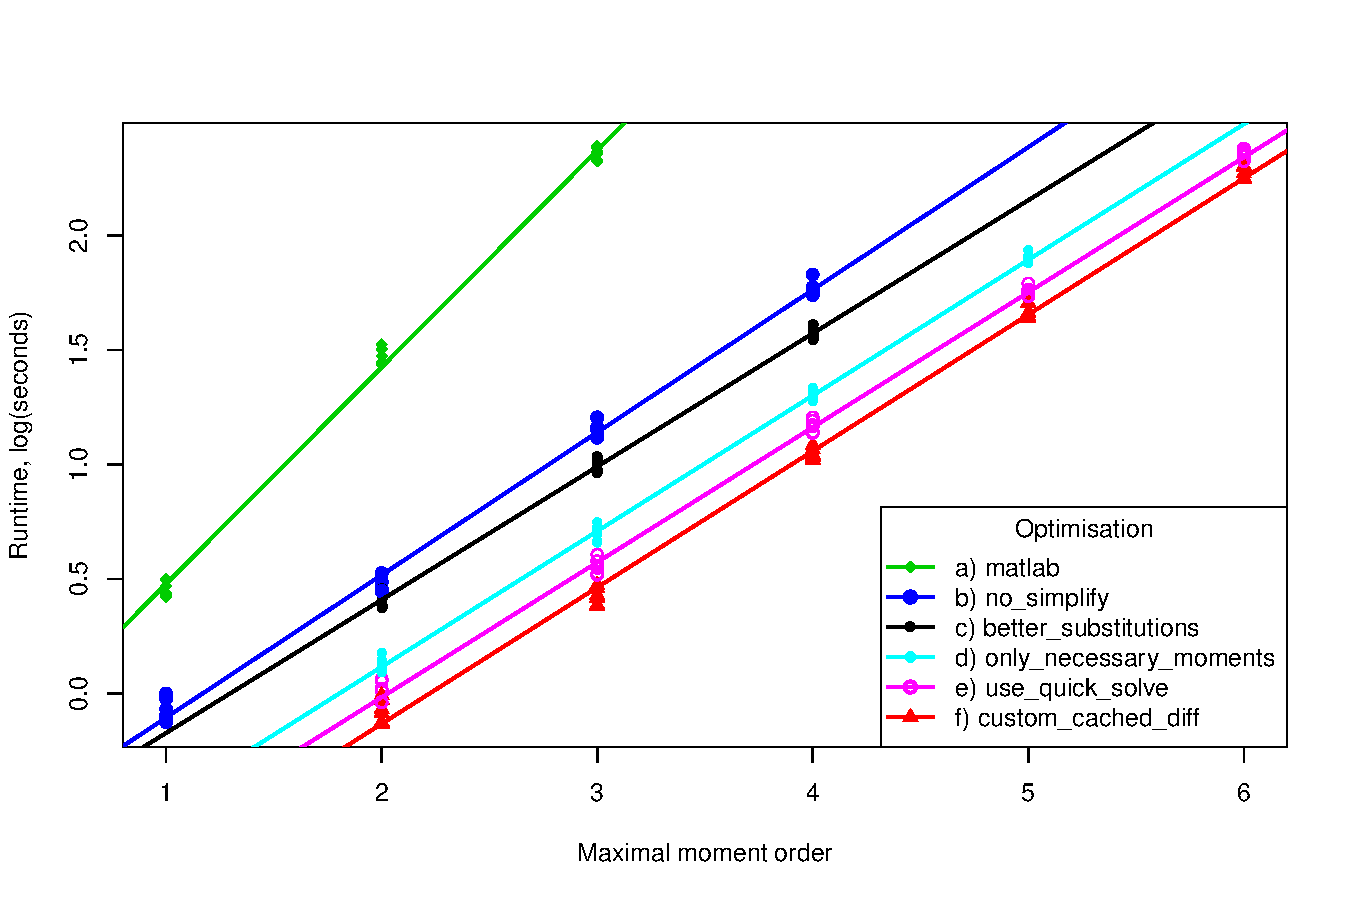
\includegraphics[width=0.95\textwidth{}]{mea_speed.pdf}
\caption{\emph{Cumulative performance improvement of symbolic 
calculations resulting from optimisation}.
The processing time for computing log-normal closure on \pft{} model with different \gls{maxord}s were measured for original Matlab implementation (a) and different optimisations (b$-$f).
In a first place, the calls to \texttt{sympy.simplify()} were removed (b). 
Then, \texttt{sympy.xreplace()} was used instead of \texttt{sympy.substitute()} (c). 
Computing a rectangular matrix containing expressions for all moment was more efficient than generating a square matrix to later remove unneeded expressions (d).
Implementing a simplified equation solver instead of using \texttt{sympy.solve()} also resulted in a significant speed-up (e). 
Finally, caching (memorisation) \texttt{sympy.diff()} allowed even better performance.
The time complexity appears exponential ($O(2^k)$, where $k$ is the maximal moments order) in every case, 
Nine replicates were performed on the same CPU. 
For optimisation c$-$f, values corresponding to \gls{maxord} moments lower than two were removed because of
the inherent inaccuracy in measuring very short durations.}
\label{fig:mea_speed}
\end{figure}

Interestingly, the slopes between, optimisations a ($0.95$) and c ($0.58$), and b ($0.62$) and c were significantly different ($p-value <10^{-15}$ and $p-value = 3 \times 10^{-4}$, respectively;
t-test on the slopes of the linear regression). This indicates that optimisation c ``scales'' better that b and a.
No significant difference was found between the slopes of the subsequent optimisations (c$-$f). 
However, the intercepts were significantly smaller between each consecutive optimisations after c) ($p-value < 10^{-6}$ for all; t-test on the intercepts of the linear regression).




\section{Implementation of \acrlong{ssa}}

\newpage{}
\bibliography{report.bib}{}
\bibliographystyle{ieeetr}


\end{document}


 
